\documentclass[aspectratio=1610, 10pt]{beamer}

% ── Tema y colores ──────────────────────────────────────────
\usetheme{Madrid}
\usecolortheme{whale}
\setbeamertemplate{navigation symbols}{}
\setbeamertemplate{footline}[frame number]
\setbeamerfont{frametitle}{size=\large, series=\bfseries}

% ── Paquetes ────────────────────────────────────────────────
\usepackage[utf8]{inputenc}
\usepackage[T1]{fontenc}
\usepackage{amsmath, amssymb, amsthm}
\usepackage{tikz}
\usetikzlibrary{automata, positioning, arrows.meta, calc, decorations.pathreplacing, shapes.geometric}
\usepackage{booktabs}
\usepackage{xcolor}
\usepackage{mathtools}
\usepackage{multicol}
\usepackage{ragged2e}

% ── Colores personalizados ──────────────────────────────────
\definecolor{accentblue}{RGB}{0,102,204}
\definecolor{accentred}{RGB}{204,0,51}
\definecolor{accentgreen}{RGB}{0,153,76}
\definecolor{softgray}{RGB}{240,240,240}
\definecolor{darktext}{RGB}{51,51,51}
\definecolor{accentorange}{RGB}{230,130,0}
\definecolor{accentpurple}{RGB}{128,0,128}

% ── Estilos de bloques ─────────────────────────────────────
\setbeamercolor{block title}{bg=accentblue, fg=white}
\setbeamercolor{block body}{bg=softgray, fg=darktext}
\setbeamercolor{block title example}{bg=accentgreen, fg=white}
\setbeamercolor{block body example}{bg=softgray, fg=darktext}
\setbeamercolor{block title alerted}{bg=accentred, fg=white}
\setbeamercolor{block body alerted}{bg=softgray, fg=darktext}

% ── Macros ──────────────────────────────────────────────────
\newcommand{\R}{\mathbb{R}}
\newcommand{\E}{\mathbb{E}}
\newcommand{\Prob}{\mathbb{P}}
\newcommand{\bpi}{\boldsymbol{\pi}}
\newcommand{\bQ}{\mathbf{Q}}
\newcommand{\bone}{\mathbf{1}}

% ── Información del documento ──────────────────────────────
\title[CTMC: Estado Estable \& PASTA]{%
  Cadenas de Markov en Tiempo Continuo\\[4pt]
  \large Estado Estable, Ergodicidad y PASTA}
\author{Modelado de Sistemas Bajo Incertidumbre}
\date{2026}

% ═══════════════════════════════════════════════════════════
\begin{document}

% ── Portada ────────────────────────────────────────────────
\begin{frame}
  \titlepage
\end{frame}

% ── Agenda ─────────────────────────────────────────────────
\begin{frame}{Agenda}
  \begin{enumerate}
    \item Repaso r\'{a}pido: CTMC y generador infinitesimal
    \item Distribuciones l\'{i}mite y estado estable
    \item \textbf{Ergodicidad}: ?`cu\'{a}ndo existe el l\'{i}mite?
    \item Contraejemplos: cadenas que \emph{no} convergen
    \item Ejemplos de estado estable resueltos
    \item Teorema PASTA --- motivaci\'{o}n y enunciado
    \item PASTA --- demostraci\'{o}n intuitiva y condiciones
    \item Contraejemplos donde PASTA \textbf{no} aplica
    \item Problemas aplicados con PASTA
    \item Resumen y conclusiones
  \end{enumerate}
\end{frame}

% ═══════════════════════════════════════════════════════════
\section{Repaso: CTMC}
% ═══════════════════════════════════════════════════════════

\begin{frame}{Cadena de Markov en Tiempo Continuo --- Repaso}
  \begin{block}{Definici\'{o}n}
    Un proceso estoc\'{a}stico $\{X(t),\; t\ge 0\}$ con espacio de estados
    $S$ finito o numerable es una \textbf{CTMC} si:
    \[
      \Prob\!\bigl(X(t+s)=j \mid X(s)=i,\; \{X(u): 0\le u < s\}\bigr)
      = \Prob\!\bigl(X(t+s)=j \mid X(s)=i\bigr)
    \]
  \end{block}
  \vspace{6pt}
  \textbf{Ingredientes clave:}
  \begin{itemize}
    \item Tasas de transici\'{o}n $q_{ij}\ge 0$ para $i\neq j$.
    \item Tasa de salida del estado $i$: $\;q_i = \sum_{j\neq i} q_{ij}$.
    \item Tiempo de permanencia en $i$: $\;\text{Exp}(q_i)$.
  \end{itemize}
\end{frame}

% ── Generador infinitesimal ────────────────────────────────
\begin{frame}{El Generador Infinitesimal $\bQ$}
  \[
    \bQ = \begin{pmatrix}
      -q_0    & q_{01} & q_{02} & \cdots \\[3pt]
      q_{10}  & -q_1   & q_{12} & \cdots \\[3pt]
      q_{20}  & q_{21}  & -q_2  & \cdots \\[3pt]
      \vdots  & \vdots  & \vdots & \ddots
    \end{pmatrix}
  \]

  \begin{alertblock}{Propiedades fundamentales}
    \begin{itemize}
      \item Cada fila suma \textbf{cero}: $\;\displaystyle\sum_j Q_{ij}=0$.
      \item Elementos diagonales: $Q_{ii} = -q_i \le 0$.
      \item Ecuaciones de Kolmogorov: $P'(t) = P(t)\,\bQ$ \;(hacia adelante).
    \end{itemize}
  \end{alertblock}
\end{frame}

% ── Ejemplo concreto de Q ─────────────────────────────────
\begin{frame}{Ejemplo: Construir $\bQ$ desde un Diagrama}
  \begin{columns}[T]
    \begin{column}{0.45\textwidth}
      \begin{center}
        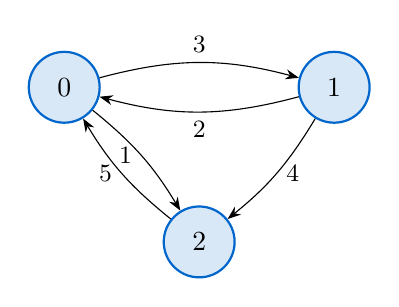
\begin{tikzpicture}[->, >=Stealth, node distance=2.5cm,
            every state/.style={fill=accentblue!15, draw=accentblue,
            thick, minimum size=0.9cm}]
          \node[state] (0) {$0$};
          \node[state, right=of 0] (1) {$1$};
          \node[state, below=1.5cm of $(0)!0.5!(1)$] (2) {$2$};
          \path (0) edge[bend left=15] node[above]{\small$3$} (1)
                (1) edge[bend left=15] node[below]{\small$2$} (0)
                (0) edge[bend left=10] node[left]{\small$1$} (2)
                (1) edge[bend left=10] node[right]{\small$4$} (2)
                (2) edge[bend left=10] node[left]{\small$5$} (0);
        \end{tikzpicture}
      \end{center}
    \end{column}
    \begin{column}{0.52\textwidth}
      \[
        \bQ = \begin{pmatrix}
          -4 & 3 & 1 \\
          2 & -6 & 4 \\
          5 & 0 & -5
        \end{pmatrix}
      \]
      \vspace{6pt}
      \textbf{Lectura:}
      \begin{itemize}
        \item Fila 0: sale con tasa $4 = 3+1$.
        \item Fila 1: sale con tasa $6 = 2+4$.
        \item Fila 2: sale con tasa $5$, solo hacia 0.
        \item Cada fila suma 0. $\checkmark$
      \end{itemize}
    \end{column}
  \end{columns}
\end{frame}

% ═══════════════════════════════════════════════════════════
\section{Distribuci\'{o}n L\'{i}mite y Estado Estable}
% ═══════════════════════════════════════════════════════════

\begin{frame}{?`Qu\'{e} Significa ``Estado Estable''?}
  Queremos saber: si dejamos evolucionar la cadena \emph{mucho} tiempo,
  ?`se estabiliza?

  \begin{block}{Distribuci\'{o}n l\'{i}mite}
    Si existen los l\'{i}mites
    \[
      \pi_j \;=\; \lim_{t\to\infty} P_{ij}(t), \qquad \forall\, i,j \in S,
    \]
    y son \textbf{independientes del estado inicial} $i$, decimos que
    $\bpi = (\pi_0, \pi_1, \ldots)$ es la \textbf{distribuci\'{o}n l\'{i}mite}
    (o de estado estable).
  \end{block}

  \vspace{6pt}
  \textbf{Interpretaci\'{o}n:}
  $\pi_j$ = fracci\'{o}n del tiempo que, a largo plazo, la cadena pasa en el estado~$j$.
\end{frame}

% ── Ecuaciones de balance ──────────────────────────────────
\begin{frame}{Ecuaciones de Balance Global}
  Si $\bpi$ existe, satisface:
  \begin{block}{Sistema de ecuaciones}
    \[
      \boxed{\;\bpi\, \bQ = \mathbf{0}\;} \qquad\text{y}\qquad
      \boxed{\;\sum_{j\in S} \pi_j = 1\;}
    \]
  \end{block}

  Escrito componente a componente:
  \[
    \sum_{i \neq j} \pi_i \, q_{ij}
    \;=\; \pi_j \, q_j, \qquad \forall\, j \in S.
  \]

  \begin{exampleblock}{Lectura intuitiva}
    \centering
    \textbf{Flujo de entrada al estado $j$} $\;=\;$
    \textbf{Flujo de salida del estado $j$}.
  \end{exampleblock}
\end{frame}

% ── Balance detallado ──────────────────────────────────────
\begin{frame}{Balance Detallado (Cadenas Reversibles)}
  Una condici\'{o}n m\'{a}s fuerte que a veces simplifica todo:
  \[
    \pi_i \, q_{ij} \;=\; \pi_j \, q_{ji}, \qquad \forall\, i \neq j.
  \]

  \begin{itemize}
    \item Se cumple en \textbf{cadenas reversibles} (colas de nacimiento--muerte).
    \item Si se verifica balance detallado, autom\'{a}ticamente se cumple
          balance global.
    \item \textbf{Truco pr\'{a}ctico:} si el grafo de transiciones es un \'{a}rbol
          o una cadena lineal, \emph{siempre} hay balance detallado.
  \end{itemize}
\end{frame}

% ── Ejemplo de balance ─────────────────────────────────────
\begin{frame}{Ejemplo: Resolver $\bpi$ para el Diagrama Anterior}
  Con $\bQ = \begin{psmallmatrix} -4 & 3 & 1 \\ 2 & -6 & 4 \\ 5 & 0 & -5 \end{psmallmatrix}$,
  resolvemos $\bpi\bQ = \mathbf{0}$:

  \vspace{4pt}
  \begin{align*}
    -4\pi_0 + 2\pi_1 + 5\pi_2 &= 0 \\
    3\pi_0 - 6\pi_1 &= 0 \;\Rightarrow\; \pi_1 = \tfrac{1}{2}\pi_0 \\
    \pi_0 + 4\pi_1 - 5\pi_2 &= 0 \;\Rightarrow\; \pi_2 = \tfrac{3}{5}\pi_0
  \end{align*}

  Con $\pi_0 + \pi_1 + \pi_2 = 1$:
  \[
    \pi_0\!\left(1 + \tfrac{1}{2} + \tfrac{3}{5}\right) = 1
    \;\Rightarrow\;
    \boxed{\pi_0 = \tfrac{10}{21},\quad \pi_1 = \tfrac{5}{21},\quad \pi_2 = \tfrac{6}{21}}
  \]

  \textbf{Verificaci\'{o}n:} la cadena es irreducible y finita $\Rightarrow$ \textbf{erg\'{o}dica}, el l\'{i}mite existe y es \'{u}nico.
\end{frame}

\begin{frame}{Ejemplo 1}
Una máquina puede estar en tres condiciones: \textbf{Operativa} (estado 0), \textbf{Degradada} (estado 1), o \textbf{Fuera de servicio} (estado 2). Las transiciones son:
\begin{itemize}
    \item De Operativa a Degradada: tasa 2 por día.
    \item De Degradada a Operativa: tasa 3 por día (reparación menor).
    \item De Degradada a Fuera de servicio: tasa 1 por día.
    \item De Fuera de servicio a Operativa: tasa 4 por día (reparación mayor).
\end{itemize}
No hay transición directa de Operativa a Fuera de servicio.

\begin{enumerate}
    \item Escriba la matriz generadora $Q$.
    \item Plantee las ecuaciones de balance y resuelva para $\pi_0, \pi_1, \pi_2$.
    \item ¿Qué fracción del tiempo está la máquina operativa?
    
\end{enumerate}

\end{frame}





\begin{frame}{Ejemplo 2}
Un estacionamiento pequeño tiene capacidad para $K = 4$ vehículos. Los vehículos llegan según un proceso de Poisson con tasa $\lambda = 10$ vehículos/hora. El tiempo que cada vehículo permanece estacionado es exponencial con media 20 minutos ($\mu = 3$ vehículos/hora).

\begin{enumerate}
    \item Identifique el modelo de colas y calcule $\rho = \lambda/\mu$ (note que $\rho > 1$; explique por qué el sistema sigue siendo estable).
    \item Calcule las probabilidades estacionarias $\pi_0, \pi_1, \pi_2, \pi_3, \pi_4$ usando la fórmula para M/M/1/K con $\rho \neq 1$.
    \item Calcule la tasa efectiva de entrada $\lambda_{\text{ef}}$.
    \item Usando la fórmula de Little ($L = \lambda_{\text{ef}} W$), calcule primero $L$ y luego $W$.
\end{enumerate}

\end{frame}

\begin{frame}{Ejemplo 3}
Una estación de bombeo tiene 2 bombas. Cada bomba falla independientemente a tasa $\alpha = 0.5$ fallas/día. Hay un solo técnico que repara bombas a tasa $\beta = 3$ reparaciones/día (una a la vez). El estado $X$ es el \textbf{número de bombas funcionando}: $X \in \{0, 1, 2\}$.

\begin{enumerate}
    \item Escriba las tasas de transición entre estados y construya el generador $Q$.
    
    \item Resuelva las ecuaciones de balance a mano para encontrar $\pi_0, \pi_1, \pi_2$.
    
    \item El caudal de agua bombeada depende del número de bombas:
    \begin{center}
    \begin{tabular}{|c|c|}
    \hline
    Bombas operativas & Caudal (litros/hora) \\
    \hline
    0 & 0 \\
    1 & 800 \\
    2 & 1500 \\
    \hline
    \end{tabular}
    \end{center}
    \emph{Nota:} el caudal no es lineal porque hay pérdidas de eficiencia con una sola bomba.
    
    Defina $Y = g(X)$ como el caudal. Calcule $E[Y]$, $\text{Var}(Y)$, y la desviación estándar.
    
    \item La comunidad requiere un caudal mínimo de 500 litros/hora. ¿Cuál es la probabilidad de no cumplir este requerimiento?
    
    \item Cada litro/hora bombeado genera \$2 de ingreso. El costo de mantener el técnico es \$1.200/día. ¿Cuál es la utilidad diaria esperada (ingreso $-$ costo del técnico)?
    
    \item Si se contrata un segundo técnico (mismo $\beta = 3$/día), las reparaciones cuando hay 2 bombas dañadas se hacen a tasa $2\beta = 6$/día. Recalcule $\pi_0, \pi_1, \pi_2$ y determine si la utilidad mejora. El segundo técnico cuesta \$1.200/día adicionales.
\end{enumerate}

\end{frame}

\begin{frame}[t]{Caso Notaría 5}
\footnotesize
\justifying

Las notarías son las instituciones que dan cuenta de la fe pública para la autenticación de actos y hechos. Recientemente, en Bogotá ha habido un aumento en el número de tramites de escrituración notariales, razón por la cual se desea analizar esta área en la notaría 5. Se sabe que la llegada de tramites a dicha notaria se comporta como un proceso de Poisson con tasa de $\gamma$ trámites/hora, de los cuales $p\%$ son de escrituración.

\vspace{0.3em}

Todo tramite de escrituración consta de dos partes, una en donde se autentica y firma el documento, y otra donde se liquida el trámite realizado. En la primera parte se verifica la validez del trámite y autentica la identidad de los involucrados en el mismo, en cuanto que, en la segunda se realiza el pago del proceso realizado. En promedio, un trámite tarda $\mu$ horas en la primera parte y $\theta$ horas en la segunda. La notaria ha dispuesto $k$ funcionarios para atender tramites en la primera parte y $m$ cajas para realizar el pago en la segunda parte. El $r\%$ de los tramites que están en proceso de liquidación deben volver a autenticarse. Esto, en su mayoría, se debe a falta de información en el documento (firmas, huellas y otros).

\vspace{0.3em}

Dado que los tramites de escrituración deben realizarse personalmente, la notaría ha designado que en un momento dado solo pueden haber $N$ tramites en proceso.

\vspace{0.3em}

Formule un modelo que le permita estudiar la ocupación del área de escrituración de la notaría 5 a lo largo del tiempo. Según el caso encuentre la matriz generadora y/o matriz de transición.

\vspace{0.3em}

Formule una expresión para determinar el valor esperado del número de tramites que hay en la 5 hora después de abierta la notaría.

\vspace{0.3em}

Formule una expresión para determinar el valor esperado del número de tramites en el largo plazo.

\end{frame}

% ═══════════════════════════════════════════════════════════
\section{Comunicaci\'{o}n entre Estados}
% ═══════════════════════════════════════════════════════════

\begin{frame}{Accesibilidad y Comunicaci\'{o}n}
  \begin{block}{Definiciones}
    \begin{itemize}
      \item El estado $j$ es \textbf{accesible} desde $i$ (escribimos $i \to j$) si
            $\exists\, t > 0$ tal que $P_{ij}(t) > 0$.

            Es decir, hay una secuencia de transiciones con tasa positiva de $i$ a $j$.
      \item Dos estados \textbf{se comunican} ($i \leftrightarrow j$) si $i \to j$ \textbf{y} $j \to i$.
    \end{itemize}
  \end{block}

  \vspace{4pt}
  \begin{exampleblock}{Propiedad clave}
    La relaci\'{o}n ``se comunican'' ($\leftrightarrow$) es de \textbf{equivalencia}:
    \begin{itemize}
      \item \textbf{Reflexiva:} $i \leftrightarrow i$ (trivialmente).
      \item \textbf{Sim\'{e}trica:} $i \leftrightarrow j \Rightarrow j \leftrightarrow i$.
      \item \textbf{Transitiva:} $i \leftrightarrow j$ y $j \leftrightarrow k$ $\Rightarrow$ $i \leftrightarrow k$.
    \end{itemize}
  \end{exampleblock}
\end{frame}

% ── Clases de comunicación ─────────────────────────────────
\begin{frame}{Clases de Comunicaci\'{o}n}
  La relaci\'{o}n $\leftrightarrow$ particiona $S$ en \textbf{clases de comunicaci\'{o}n}:
  conjuntos maximales de estados que se comunican entre s\'{i}.

  \begin{columns}[T]
    \begin{column}{0.48\textwidth}
      \begin{center}
        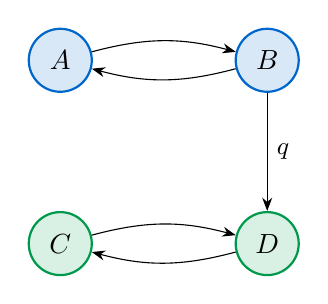
\begin{tikzpicture}[->, >=Stealth, node distance=1.8cm,
            every state/.style={thick, minimum size=0.8cm}]
          % Clase 1
          \node[state, fill=accentblue!15, draw=accentblue] (A) {$A$};
          \node[state, fill=accentblue!15, draw=accentblue, right=of A] (B) {$B$};
          % Clase 2
          \node[state, fill=accentgreen!15, draw=accentgreen, below=1.5cm of A] (C) {$C$};
          \node[state, fill=accentgreen!15, draw=accentgreen, right=of C] (D) {$D$};
          \path (A) edge[bend left=15] (B)
                (B) edge[bend left=15] (A)
                (C) edge[bend left=15] (D)
                (D) edge[bend left=15] (C)
                (B) edge node[right]{\small$q$} (D);
        \end{tikzpicture}

        {\small Clase azul: $\{A,B\}$, Clase verde: $\{C,D\}$.}
      \end{center}
    \end{column}
    \begin{column}{0.50\textwidth}
      \begin{itemize}
        \item $A \leftrightarrow B$: se comunican (flechas en ambos sentidos).
        \item $C \leftrightarrow D$: se comunican.
        \item $B \to D$ pero $D \not\to B$: \textbf{no} se comunican.
        \item $\{A,B\}$ \textbf{no es cerrada}: puede salir ($B \to D$).
        \item $\{C,D\}$ \textbf{es cerrada}: no hay salida.
      \end{itemize}
    \end{column}
  \end{columns}
\end{frame}

% ── Clases cerradas e irreducibilidad ─────────────────────
\begin{frame}{Clases Cerradas e Irreducibilidad}
  \begin{block}{Clase cerrada (absorbente)}
    Una clase de comunicaci\'{o}n $C \subseteq S$ es \textbf{cerrada} si
    ning\'{u}n estado de $C$ tiene transici\'{o}n hacia un estado fuera de $C$:
    \[
      q_{ij} = 0 \quad \forall\, i \in C,\; j \notin C.
    \]
    Una vez que la cadena entra en $C$, nunca sale.
  \end{block}

  \begin{block}{Cadena irreducible}
    Una CTMC es \textbf{irreducible} si tiene \textbf{una sola clase de comunicaci\'{o}n},
    es decir, $i \leftrightarrow j$ para todos $i, j \in S$.

    Equivalentemente: desde cualquier estado se puede llegar a cualquier otro.
  \end{block}

  \vspace{4pt}
  \textbf{?`Por qu\'{e} importa?} Solo las cadenas irreducibles (o restringidas a una clase cerrada)
  pueden tener una distribuci\'{o}n l\'{i}mite \'{u}nica independiente del estado inicial.
\end{frame}

% ── Ejemplo visual de comunicación ─────────────────────────
\begin{frame}{Ejemplo: Identificar Clases de Comunicaci\'{o}n}
  \begin{center}
    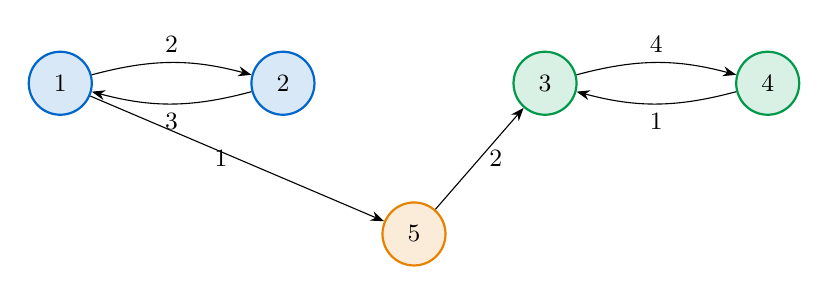
\begin{tikzpicture}[->, >=Stealth, node distance=2cm,
        every state/.style={thick, minimum size=0.8cm, font=\small}]
      \node[state, fill=accentblue!15, draw=accentblue] (1) {$1$};
      \node[state, fill=accentblue!15, draw=accentblue, right=of 1] (2) {$2$};
      \node[state, fill=accentgreen!15, draw=accentgreen, right=2.5cm of 2] (3) {$3$};
      \node[state, fill=accentgreen!15, draw=accentgreen, right=of 3] (4) {$4$};
      \node[state, fill=accentorange!15, draw=accentorange, below=1.5cm of $(2)!0.5!(3)$] (5) {$5$};
      \path (1) edge[bend left=15] node[above]{\small$2$} (2)
            (2) edge[bend left=15] node[below]{\small$3$} (1)
            (3) edge[bend left=15] node[above]{\small$4$} (4)
            (4) edge[bend left=15] node[below]{\small$1$} (3)
            (1) edge node[left]{\small$1$} (5)
            (5) edge node[right]{\small$2$} (3);
    \end{tikzpicture}
  \end{center}

  \begin{itemize}
    \item \textcolor{accentblue}{\textbf{Clase $\{1,2\}$}}: $1 \leftrightarrow 2$. \textbf{No cerrada} (se puede salir: $1 \to 5$).
    \item \textcolor{accentorange}{\textbf{Clase $\{5\}$}}: estado solo. \textbf{No cerrada} ($5 \to 3$).
    \item \textcolor{accentgreen}{\textbf{Clase $\{3,4\}$}}: $3 \leftrightarrow 4$. \textbf{Cerrada} (no hay salida).
    \item La cadena \textbf{no} es irreducible. A largo plazo, la cadena termina atrapada en $\{3,4\}$.
  \end{itemize}
\end{frame}

% ═══════════════════════════════════════════════════════════
\section{Recurrencia y Transitoriedad}
% ═══════════════════════════════════════════════════════════

\begin{frame}{Recurrencia: ?`La Cadena Regresa?}
  \begin{block}{Definici\'{o}n intuitiva}
    Sea $T_i = \inf\{t > 0 : X(t) = i \mid X(0) = i\}$ el primer tiempo de retorno al estado $i$
    (despu\'{e}s de haberlo dejado).
    \begin{itemize}
      \item Estado $i$ es \textbf{recurrente} si $\Prob(T_i < \infty) = 1$:
            la cadena \textbf{siempre regresa} a $i$.
      \item Estado $i$ es \textbf{transitorio} si $\Prob(T_i < \infty) < 1$:
            hay probabilidad positiva de \textbf{nunca regresar}.
    \end{itemize}
  \end{block}

  \vspace{6pt}
  \begin{alertblock}{Propiedad de clase}
    La recurrencia/transitoriedad es una propiedad de \textbf{clase}:
    si $i$ es recurrente y $i \leftrightarrow j$, entonces $j$ tambi\'{e}n es recurrente.
    Lo mismo para transitoriedad.
  \end{alertblock}
\end{frame}

% ── Criterio de recurrencia ────────────────────────────────
\begin{frame}{Criterio de Recurrencia}
  \begin{block}{Criterio integral}
    Un estado $i$ es \textbf{recurrente} si y solo si:
    \[
      \int_0^{\infty} P_{ii}(t)\, dt = \infty
    \]
    y es \textbf{transitorio} si y solo si esta integral es finita.
  \end{block}

  \vspace{4pt}
  \textbf{Interpretaci\'{o}n:} $P_{ii}(t)$ mide la probabilidad de estar en $i$ al tiempo $t$.
  Si la integral diverge, la cadena ``pasa tiempo infinito'' volviendo a $i$.

  \vspace{6pt}
  \begin{exampleblock}{Consecuencia para espacios finitos}
    Si $S$ es \textbf{finito} y la cadena es \textbf{irreducible}, entonces
    \textbf{todos} los estados son recurrentes. (No hay d\'{o}nde ``escapar''.)
  \end{exampleblock}
\end{frame}

% ── Recurrencia positiva vs nula ──────────────────────────
\begin{frame}{Recurrencia Positiva vs.\ Recurrencia Nula}
  Dentro de los estados recurrentes, hay una distinci\'{o}n crucial:

  \vspace{4pt}
  \begin{columns}[T]
    \begin{column}{0.48\textwidth}
      \begin{block}{Recurrente positivo}
        \begin{itemize}
          \item $\E[T_i] < \infty$: el tiempo medio de retorno es \textbf{finito}.
          \item La cadena regresa ``r\'{a}pido'' en promedio.
          \item Permite definir $\pi_i = 1/\E[T_i] > 0$.
        \end{itemize}
      \end{block}
    \end{column}
    \begin{column}{0.48\textwidth}
      \begin{alertblock}{Recurrente nulo}
        \begin{itemize}
          \item $\E[T_i] = \infty$: el tiempo medio de retorno es \textbf{infinito}.
          \item La cadena regresa, pero tarda ``demasiado''.
          \item $\pi_i = 1/\E[T_i] = 0$: no se puede normalizar.
        \end{itemize}
      \end{alertblock}
    \end{column}
  \end{columns}

  \vspace{8pt}
  \begin{exampleblock}{Hecho clave}
    Para cadenas irreducibles con $S$ \textbf{finito}:
    recurrente $\Rightarrow$ \textbf{recurrente positivo} siempre.

    La recurrencia nula solo ocurre con espacios de estados infinitos.
  \end{exampleblock}
\end{frame}

% ── Transitoriedad visual ─────────────────────────────────
\begin{frame}{Transitoriedad: La Cadena No Regresa}
  \begin{center}
    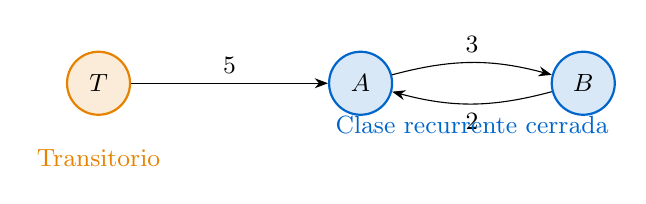
\begin{tikzpicture}[->, >=Stealth, node distance=2cm,
        every state/.style={thick, minimum size=0.8cm, font=\small}]
      % Estado transitorio
      \node[state, fill=accentorange!15, draw=accentorange] (T) {$T$};
      % Clase recurrente
      \node[state, fill=accentblue!15, draw=accentblue, right=2.5cm of T] (A) {$A$};
      \node[state, fill=accentblue!15, draw=accentblue, right=of A] (B) {$B$};
      \path (T) edge node[above]{\small$5$} (A)
            (A) edge[bend left=15] node[above]{\small$3$} (B)
            (B) edge[bend left=15] node[below]{\small$2$} (A);
      % Label
      \node[below=0.3cm of T, text=accentorange] {\small Transitorio};
      \node[below=0.3cm of $(A)!0.5!(B)$, text=accentblue] {\small Clase recurrente cerrada};
    \end{tikzpicture}
  \end{center}

  \begin{itemize}
    \item El estado $T$ es \textbf{transitorio}: una vez que sale hacia $A$, \textbf{nunca regresa}.
    \item $\{A, B\}$ es una clase cerrada recurrente.
    \item A largo plazo, $\pi_T = 0$: la cadena abandona los estados transitorios para siempre.
  \end{itemize}

  \vspace{4pt}
  \begin{block}{Regla general}
    En estado estable, los estados transitorios tienen probabilidad \textbf{cero}.
    Toda la masa de probabilidad se concentra en las clases recurrentes cerradas.
  \end{block}
\end{frame}

% ── Resumen jerarquía de conceptos ─────────────────────────
\begin{frame}{Jerarqu\'{i}a de Conceptos: Del Estado a la Ergodicidad}
  \begin{center}
    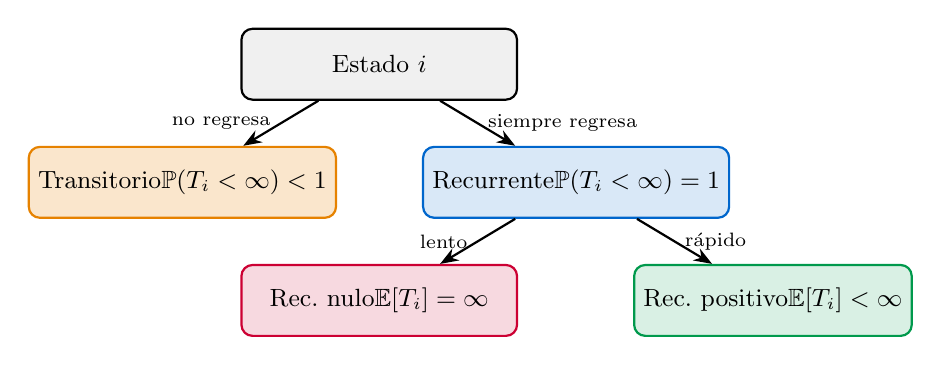
\begin{tikzpicture}[
      every node/.style={draw, rounded corners, thick, text centered,
        minimum width=3.5cm, minimum height=0.9cm, font=\small},
      level 1/.style={sibling distance=5cm},
      ->, >=Stealth, thick
    ]
      \node[fill=softgray] (est) {Estado $i$}
        child {node[fill=accentorange!20, draw=accentorange] (trans) {Transitorio\\$\Prob(T_i<\infty)<1$}
          edge from parent node[left, draw=none, font=\scriptsize, minimum width=0cm] {no regresa}}
        child {node[fill=accentblue!15, draw=accentblue] (rec) {Recurrente\\$\Prob(T_i<\infty)=1$}
          child {node[fill=accentred!15, draw=accentred] (nul) {Rec.\ nulo\\$\E[T_i]=\infty$}
            edge from parent node[left, draw=none, font=\scriptsize, minimum width=0cm] {lento}}
          child {node[fill=accentgreen!15, draw=accentgreen] (pos) {Rec.\ positivo\\$\E[T_i]<\infty$}
            edge from parent node[right, draw=none, font=\scriptsize, minimum width=0cm] {r\'{a}pido}}
          edge from parent node[right, draw=none, font=\scriptsize, minimum width=0cm] {siempre regresa}};
    \end{tikzpicture}
  \end{center}

  \vspace{6pt}
  \begin{block}{Para ergodicidad necesitamos:}
  \begin{enumerate}
    \item Cadena \textbf{irreducible} (una sola clase de comunicaci\'{o}n).
    \item Todos los estados \textbf{recurrentes positivos}.
  \end{enumerate}
  En CTMCs, la periodicidad \textbf{no} es problema (tiempos continuos la rompen).
  \end{block}
\end{frame}

% ═══════════════════════════════════════════════════════════
\section{Ergodicidad}
% ═══════════════════════════════════════════════════════════

\begin{frame}{?`Siempre Existe el L\'{i}mite?{} --- La Pregunta Clave}
  \begin{alertblock}{Respuesta corta: NO}
    No toda CTMC tiene distribuci\'{o}n l\'{i}mite. Necesitamos
    condiciones adicionales.
  \end{alertblock}

  \vspace{4pt}
  Problemas posibles (ahora con el vocabulario correcto):
  \begin{enumerate}
    \item \textbf{Reducibilidad}: hay m\'{u}ltiples clases cerradas ---
          el l\'{i}mite depende del estado inicial.
    \item \textbf{Transitoriedad}: existen estados (o clases) de los que
          la cadena se ``escapa'' y no regresa.
    \item \textbf{Recurrencia nula}: la cadena regresa a cada estado, pero el tiempo medio
          de retorno es infinito $\Rightarrow$ no se puede normalizar $\bpi$.
  \end{enumerate}

  \vspace{4pt}
  \textbf{Nota:} la periodicidad, que es problema en DTMCs, \textbf{no} afecta
  a CTMCs porque los tiempos exponenciales ``rompen'' cualquier ciclo.
\end{frame}

% ── Condiciones de ergodicidad ─────────────────────────────
\begin{frame}{Teorema de Ergodicidad para CTMCs}
  \begin{block}{Teorema}
    Sea $\{X(t)\}$ una CTMC \textbf{irreducible}. Entonces:
    \begin{enumerate}
      \item Si $S$ es \textbf{finito}: la cadena es \textbf{siempre erg\'{o}dica}.
            Existe una \'{u}nica $\bpi > \mathbf{0}$ con $\bpi\bQ = \mathbf{0}$,
            $\sum \pi_j = 1$.
      \item Si $S$ es \textbf{infinito numerable}: la cadena es erg\'{o}dica
            \textbf{si y solo si} es recurrente positiva, lo cual equivale a que
            $\bpi\bQ = \mathbf{0}$ tenga soluci\'{o}n con $\sum_j \pi_j = 1$.
    \end{enumerate}
  \end{block}

  \vspace{6pt}
  \textbf{?`Por qu\'{e} no hay condici\'{o}n de aperiodicidad?}

  En DTMCs se requiere aperiodicidad. En CTMCs, el tiempo de permanencia
  $\text{Exp}(q_i)$ es continuo, as\'{i} que la cadena puede ``regresar'' a cualquier
  estado en cualquier instante $t > 0$. Los ciclos peri\'{o}dicos no pueden formarse.
\end{frame}

% ── Irreducibilidad visual ────────────────────────────────
\begin{frame}{Irreducibilidad: Todos Se Comunican}
  \begin{columns}[T]
    \begin{column}{0.48\textwidth}
      \textbf{Irreducible} $\checkmark$

      \begin{center}
        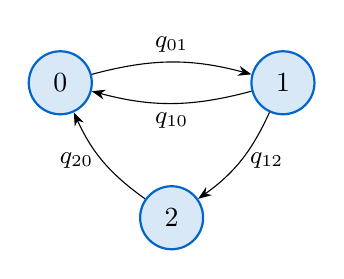
\begin{tikzpicture}[->, >=Stealth, node distance=2cm,
            every state/.style={fill=accentblue!15, draw=accentblue,
            thick, minimum size=0.8cm}]
          \node[state] (0) {$0$};
          \node[state, right=of 0] (1) {$1$};
          \node[state, below=1.3cm of $(0)!0.5!(1)$] (2) {$2$};
          \path (0) edge[bend left=15] node[above]{\small$q_{01}$} (1)
                (1) edge[bend left=15] node[below]{\small$q_{10}$} (0)
                (1) edge[bend left=15] node[right]{\small$q_{12}$} (2)
                (2) edge[bend left=15] node[left]{\small$q_{20}$} (0);
        \end{tikzpicture}
      \end{center}
      Una sola clase: $\{0,1,2\}$.

      Todos se comunican entre s\'{i}.
    \end{column}
    \begin{column}{0.48\textwidth}
      \textbf{Reducible} $\boldsymbol{\times}$

      \begin{center}
        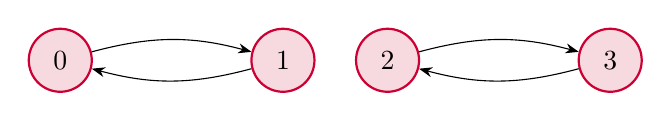
\begin{tikzpicture}[->, >=Stealth, node distance=2cm,
            every state/.style={fill=accentred!15, draw=accentred,
            thick, minimum size=0.8cm}]
          \node[state] (0) {$0$};
          \node[state, right=of 0] (1) {$1$};
          \node[state, right=0.5cm of 1] (2) {$2$};
          \node[state, right=of 2] (3) {$3$};
          \path (0) edge[bend left=15] (1)
                (1) edge[bend left=15] (0)
                (2) edge[bend left=15] (3)
                (3) edge[bend left=15] (2);
        \end{tikzpicture}
      \end{center}
      Dos clases cerradas: $\{0,1\}$ y $\{2,3\}$.

      No hay comunicaci\'{o}n entre ellas.
    \end{column}
  \end{columns}
\end{frame}

% ── Contraejemplo 1: Reducible ────────────────────────────
\begin{frame}{Contraejemplo 1: Cadena Reducible --- L\'{i}mite Depende del Inicio}
  \begin{center}
    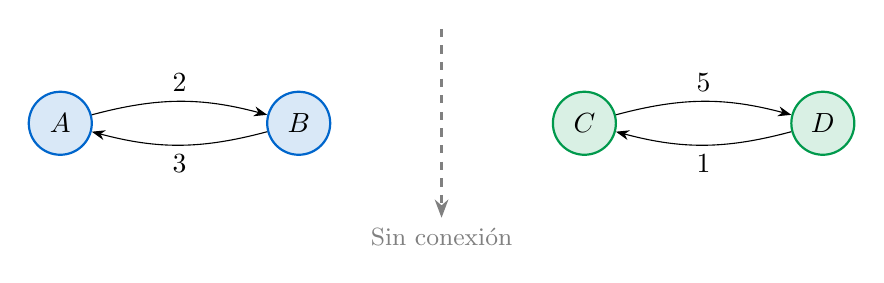
\begin{tikzpicture}[->, >=Stealth, node distance=2.2cm,
        every state/.style={thick, minimum size=0.8cm}]
      \node[state, fill=accentblue!15, draw=accentblue] (A) {$A$};
      \node[state, fill=accentblue!15, draw=accentblue, right=of A] (B) {$B$};
      \node[state, fill=accentgreen!15, draw=accentgreen, right=2.8cm of B] (C) {$C$};
      \node[state, fill=accentgreen!15, draw=accentgreen, right=of C] (D) {$D$};
      \path (A) edge[bend left=15] node[above]{$2$} (B)
            (B) edge[bend left=15] node[below]{$3$} (A)
            (C) edge[bend left=15] node[above]{$5$} (D)
            (D) edge[bend left=15] node[below]{$1$} (C);
      \draw[dashed, thick, gray] ($(B.east)!0.5!(C.west)$) ++(0,1.2) --
            ++(0,-2.4) node[below, text=gray]{\small Sin conexi\'{o}n};
    \end{tikzpicture}
  \end{center}

  \begin{itemize}
    \item Dos clases cerradas de comunicaci\'{o}n: $\{A,B\}$ y $\{C,D\}$.
    \item Si empiezo en $A$: $\;\bpi = (3/5,\; 2/5,\; 0,\; 0)$.
    \item Si empiezo en $C$: $\;\bpi = (0,\; 0,\; 1/6,\; 5/6)$.
    \item \textbf{El l\'{i}mite depende del estado inicial}
          $\Rightarrow$ \textbf{no hay ergodicidad}.
    \item \textbf{Diagn\'{o}stico:} falla la \textbf{irreducibilidad}.
  \end{itemize}
\end{frame}

% ── Contraejemplo 2: Estado absorbente ────────────────────
\begin{frame}{Contraejemplo 2: Estado Absorbente}
  \begin{center}
    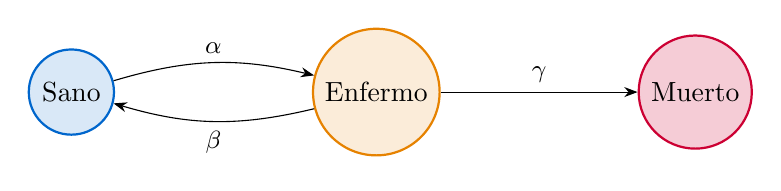
\begin{tikzpicture}[->, >=Stealth, node distance=2.5cm,
        every state/.style={thick, minimum size=0.9cm}]
      \node[state, fill=accentblue!15, draw=accentblue] (0) {Sano};
      \node[state, fill=accentorange!15, draw=accentorange, right=of 0] (1) {Enfermo};
      \node[state, fill=accentred!20, draw=accentred, right=of 1] (2) {Muerto};
      \path (0) edge[bend left=15] node[above]{\small$\alpha$} (1)
            (1) edge[bend left=15] node[below]{\small$\beta$} (0)
            (1) edge node[above]{\small$\gamma$} (2);
    \end{tikzpicture}
  \end{center}

  \begin{itemize}
    \item ``Muerto'' es un \textbf{estado absorbente}: $q_{2,j}=0$ para todo $j$. Forma su propia clase cerrada $\{2\}$.
    \item Clases: $\{$Sano, Enfermo$\}$ (no cerrada, transitoria) y $\{$Muerto$\}$ (cerrada).
    \item $\lim_{t\to\infty} \Prob(X(t)=\text{Muerto}) = 1$, independiente del inicio.
    \item $\bpi = (0, 0, 1)$ es degenerada.
    \item \textbf{Diagn\'{o}stico:} no irreducible. Los estados ``Sano'' y ``Enfermo'' son \textbf{transitorios}.
  \end{itemize}
\end{frame}

% ── Contraejemplo 3: Trampa de absorción ─────────────────
\begin{frame}{Contraejemplo 3: Bacteria --- ?`Trampa de Absorci\'{o}n!}
  \begin{exampleblock}{Enunciado}
    \small
    Cada bacteria se divide a tasa $\lambda = 2$/h y muere a tasa $\mu = 3$/h
    (tasas por bacteria). Se empieza con 1. ?`Existe estado estable?
  \end{exampleblock}

  \textbf{Modelo:} nacimiento--muerte con $\lambda_n = 2n$, $\mu_n = 3n$.

  $\lambda_n / \mu_n = 2/3 < 1$, parece estable...

  \vspace{4pt}
  \textbf{Pero:} $\mu_0 = 0$ y $\lambda_0 = 0$. El estado $0$ es \textbf{absorbente}.

  \begin{alertblock}{Resultado}
    $\Prob(X(t)=0) \to 1$. La poblaci\'{o}n se extingue.

    \textbf{Diagn\'{o}stico:} la cadena \textbf{no es irreducible}. El estado 0 es una clase cerrada separada.
    Los dem\'{a}s estados ($1, 2, 3, \ldots$) son \textbf{transitorios}.

    \textbf{Moraleja:} verificar comunicaci\'{o}n e irreducibilidad \textbf{antes} de calcular $\rho$.
  \end{alertblock}
\end{frame}

% ── Resumen ergodicidad ───────────────────────────────────
\begin{frame}{Resumen: ?`Cu\'{a}ndo Puedo Calcular $\bpi$?}
  \begin{center}
    \renewcommand{\arraystretch}{1.5}
    \begin{tabular}{lcc}
      \toprule
      \textbf{Condici\'{o}n} & \textbf{$|S|$ finito} & \textbf{$|S|$ infinito} \\
      \midrule
      Irreducible & Siempre erg\'{o}dica & Depende (rec.\ positiva?) \\
      Reducible & L\'{i}mite depende de $X(0)$ & L\'{i}mite depende de $X(0)$ \\
      Rec.\ positiva & Siempre (si irred.) & $\Leftrightarrow$ erg\'{o}dica \\
      Rec.\ nula & No ocurre (finito) & No hay $\bpi$ sumable \\
      Transitoria & No ocurre (si irred.) & No hay $\bpi$ \\
      \bottomrule
    \end{tabular}
  \end{center}

  \begin{block}{Receta pr\'{a}ctica para esta clase}
    \begin{enumerate}
      \item Identificar las \textbf{clases de comunicaci\'{o}n} y verificar \textbf{irreducibilidad}.
      \item Si $S$ es finito e irreducible: $\bpi$ \textbf{existe y es \'{u}nica}. Resolver directamente.
      \item Si $S$ es infinito: verificar condici\'{o}n de estabilidad (e.g., $\lambda < \mu$).
      \item Resolver $\bpi\bQ = \mathbf{0}$, $\;\sum \pi_j = 1$.
    \end{enumerate}
  \end{block}
\end{frame}


\end{document}

